\documentclass[10pt]{article}
\usepackage[margin=0.8in]{geometry}
\usepackage[utf8]{inputenc}
\usepackage[T1]{fontenc}
\usepackage{graphicx}
\usepackage[export]{adjustbox}
\usepackage{amsmath}
\usepackage{amsfonts}
\usepackage{amssymb}
\usepackage[version=4]{mhchem}
\usepackage{stmaryrd}
\usepackage{bbold}
\usepackage{fixltx2e}
\usepackage{caption}
\usepackage{mathtools}
\usepackage[parfill]{parskip}
\usepackage{float}
\usepackage{amsmath}

\usepackage[framemethod=TikZ]{mdframed}
\colorlet{shadecolor}{orange!15}
\usepackage{xcolor}
\usepackage{amsthm}
\usepackage{framed}

\begin{document}


\title{Lecture 20: Decentralized Joint Control}
\author{Wanxin Jin}
\maketitle


\section{Why Decentralized Joint Control?}

The equation of motion of a manipulator without  end-effector contact force and  any joint friction is

\begin{equation}\label{equ.dyn}
    \boldsymbol{B}(\boldsymbol{q}) \ddot{\boldsymbol{q}}+\boldsymbol{C}(\boldsymbol{q}, \dot{\boldsymbol{q}}) \dot{\boldsymbol{q}}+\boldsymbol{g}(\boldsymbol{q})=\boldsymbol{\tau}
\end{equation}


Let $\boldsymbol{q}_{m}=[\theta_{m1}, \theta_{m2}, ...\theta_{mn}]^T$ denote the vector of all corresponding DM motor angles. The transmissions establish a relationship:

\begin{equation}\label{equ.motor_angle}
    \boldsymbol{K}_{r} \boldsymbol{q}=\boldsymbol{q}_{m}
\end{equation}

where $\boldsymbol{K}_{r}=\text{diag}(k_{r_1}, k_{r_2}, ..., k_{r_n})$ is a diagonal matrix, and each diagonal element $k_{r_i}$ is the gear ratio of joint $i$. Let $\boldsymbol{\tau}_{m}=[\tau_{m1},\tau_{m2},...,,\tau_{mn}]^T$ denote the vector of all motor torques, one can write

\begin{equation}\label{equ.motor_torque}
\boldsymbol{\tau}_{m}=\boldsymbol{K}_{r}^{-1} \boldsymbol{\tau}
\end{equation}


Substituting (\ref{equ.motor_angle})  and (\ref{equ.motor_torque}) into the manipulator dynamics (\ref{equ.dyn}) leads to
\begin{equation}\label{equ.dyn2}
    \boldsymbol{K}_{r}^{-1} \boldsymbol{B}(\boldsymbol{q}) \boldsymbol{K}_{r}^{-1} \ddot{\boldsymbol{q}}_{m}+\boldsymbol{K}_{r}^{-1} \boldsymbol{C}(\boldsymbol{q}, \dot{\boldsymbol{q}}) \boldsymbol{K}_{r}^{-1} \dot{\boldsymbol{q}}_{m}+\boldsymbol{K}_{r}^{-1} \boldsymbol{g}(\boldsymbol{q})=\boldsymbol{\tau}_{m}
\end{equation}
We have previously analyzed elements in matrix $\boldsymbol{B}(\boldsymbol{q})$, one can write it as
\begin{equation}\label{equ.bmat}
    \boldsymbol{B}(\boldsymbol{q})=\overline{\boldsymbol{B}}+\Delta \boldsymbol{B}(\boldsymbol{q})
\end{equation}
where $\overline{\boldsymbol{B}}$ is the diagonal matrix whose constant elements represent the average inertia at each joint, and elements in $\Delta \boldsymbol{B}(\boldsymbol{q})$ represent the matrix of  non-diagonal  part. Substituting (\ref{equ.bmat}) into (\ref{equ.dyn2}) leads to
\begin{equation}\label{equ.decouple_model}
    \underbrace{\boldsymbol{K}_{r}^{-1} \overline{\boldsymbol{B}} \boldsymbol{K}_{r}^{-1}}_{\boldsymbol{I}_m} \ddot{\boldsymbol{q}}_{m}+\underbrace{\boldsymbol{K}_{r}^{-1} \Delta \boldsymbol{B}(\boldsymbol{q}) \boldsymbol{K}_{r}^{-1} \ddot{\boldsymbol{q}}_{m}+\boldsymbol{K}_{r}^{-1} \boldsymbol{C}(\boldsymbol{q}, \dot{\boldsymbol{q}}) \boldsymbol{K}_{r}^{-1} \dot{\boldsymbol{q}}_{m}+\boldsymbol{K}_{r}^{-1} \boldsymbol{g}(\boldsymbol{q})}_{\boldsymbol{D}}=\boldsymbol{\tau}_{m}
\end{equation}
The above equation (\ref{equ.decouple_model}) will lead to the following diagram. 

\begin{figure}[H]
    \centering
    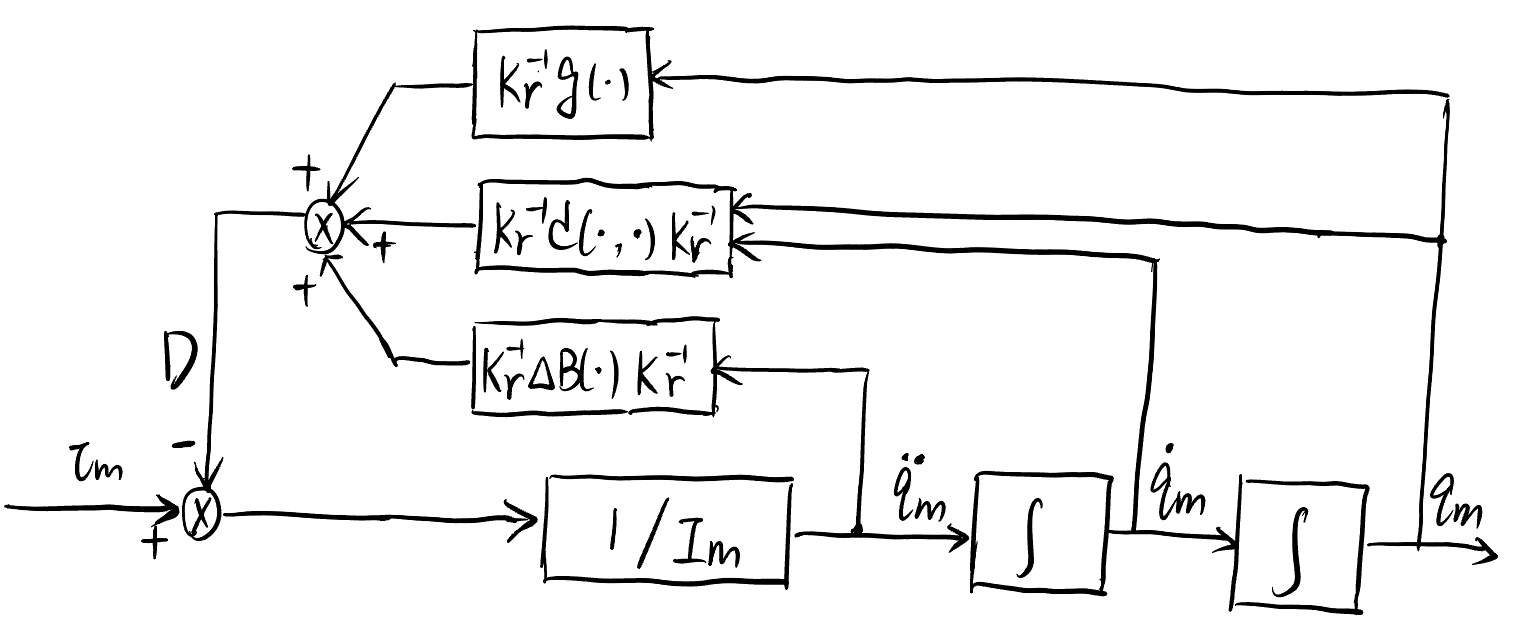
\includegraphics[max width=0.65\textwidth]{control/decentralized_control3.jpeg}
    \caption{Dynamics diagram of a motor-driven manipulator.}
    \label{fig:3}
\end{figure}

As shown in Fig. \ref{fig:3} and (\ref{equ.decouple_model}), if we don't consider $\boldsymbol{D}$, then 
$$
\boldsymbol{I}_m\boldsymbol{\ddot{q}}_m=\boldsymbol{\tau}_m,
$$
Note that in the above equation $\boldsymbol{I}_m$ is also a diagonal matrix. This means that if we don't consider the complex $\boldsymbol{D}$, each joint is a single-in-single-output system:
\begin{equation}\label{equ.single_joint_dyn}
    {I}_m{\ddot{\theta}_m}=\tau_m
\end{equation}
for each joint motor and we can control each joint individually. However, $\boldsymbol{D}$ in (\ref{equ.decouple_model}) is a coupling term that prevents us from doing so. To address such, in the following, we still consider the control each joint as a single-in-single-out system, but consider $\boldsymbol{D}$ as a disturbance to each joint.






\section{Single-Joint Control Diagram}

For each joint (we omit the joint index $i$ below), considering (\ref{equ.single_joint_dyn}) and the motor model in the previous lecture (Lecture 19), we have 
\begin{equation}\label{equ.motor}
I_m\ddot{\theta}_m+D=\tau_m=I_m\ddot{\theta}_m+\frac{k_t}{R_a}(\frac{DR_a}{k_t})=\tau_m=k_ti_a=k_t\frac{(v_a-k_v\dot{\theta}_m)}{R_a}=k_t\frac{(G_vv_c-k_v\dot{\theta}_m)}{R_a}
\end{equation}

Here, $D$ is the disturbance torque in (\ref{equ.decouple_model}) applied to each joint,  ${k}_{t}$ is the torque constants;  ${i}_{a}$ is the  armature current; $ {v}_{a}$ is the vector of armature voltage; ${R}_{a}$ is the  armature resistance; ${k}_{v}$ is the back EMF constant; $\boldsymbol{v}_{c}$ is the voltage of the servomotor, and $G_v$ is amplifier. Those motor parameters have been shown in previous lecture. In the following, we will suppose $v_c=v_a$, i.e., $G_v=1$, for notation simplicity, and so we will directly treat $v_a$ as the servo motor input voltage. But the analysis also holds for any $G_v$. 


The above (\ref{equ.motor}) corresponds to the following diagram:
\begin{figure}[H]
    \centering
    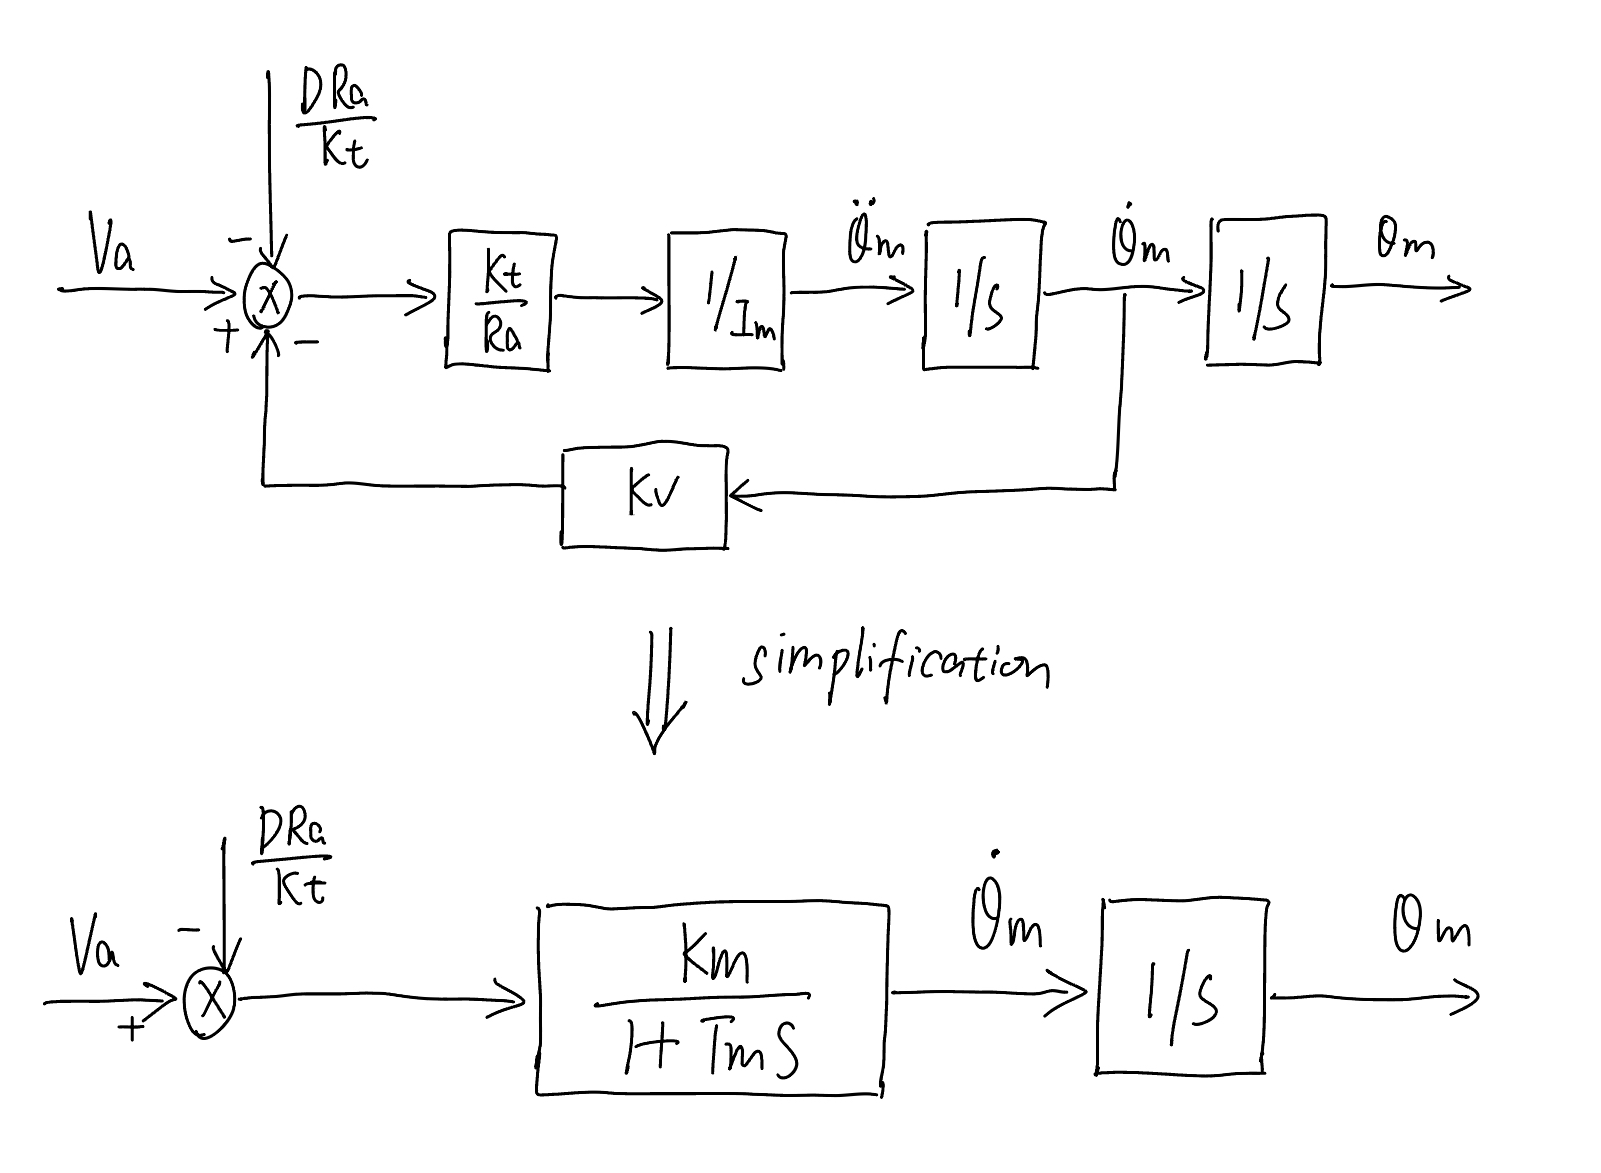
\includegraphics[max width=0.6\textwidth]{control/motor_model3.jpeg}
    \caption{Diagram of a motor-driven manipulator, with coupled joint terms treated as disturbance.}
    \label{fig:motor_model2}
\end{figure}


In the above diagram, the closed loop is due to the DC motor model itself. We write input ($V_a$) to output ($\theta_m$) transfer function
\begin{equation}\label{equ.motortf}
    G(s)=\frac{{\Theta}(s)}{V_a(s)}=\frac{k_m}{s(1+T_ms)}
\end{equation}

\begin{equation}
    \frac{\dot{\Theta}(s)}{V_a(s)}=\frac{\frac{k_t}{R_aI_ms}}{1+\frac{k_t}{R_aI_ms}k_v}=\frac{k_m}{1+T_ms}
\end{equation}

% For the diagram in Fig. \ref{fig:motor_model2}, its control diagram is in Fig. \ref{fig.general_control_diag}, where $C_{P}(s), C_{V}(s), C_{A}(s)$ respectively represent position, velocity, acceleration controllers, and $k_{T P}, k_{T V}, k_{T A}$ are the respective transducer constants (the constant for the respective sensors). Notice that $\vartheta_{r}$ is the reference input.


% \begin{figure}[H]
%     \centering
%     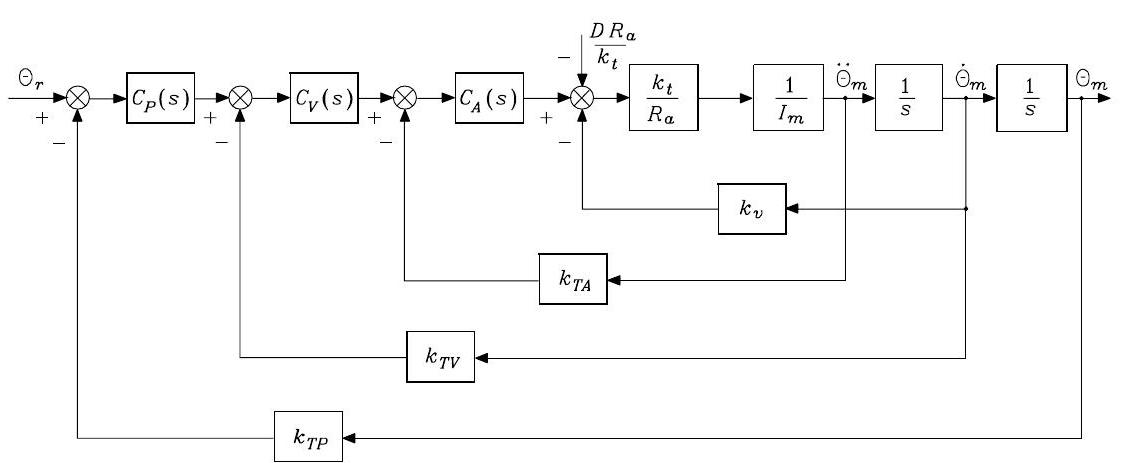
\includegraphics[max width=0.7\textwidth]{control/decentralized_control.jpg}
%     \caption{General control diagram for  decentralized joint control of a manipulator.}
%     \label{fig.general_control_diag}
% \end{figure}


\section{Minimal Control Background}

For ease of the reader, we provide the following minimal background of control design. A typical closed-loop control diagram is shown below. Here, $\theta_r$ is the reference input; $\theta_m$ is the output; $D$ is the disturbance; $G(s)$ is the transfer function of the plant to be controlled; $C(s)$ is the controller; $H(s)$ is the backward pass transfer function (usually a constant due to sensor). The goal of control design is to find $C(s)$ such that $\theta_m$ is able to track $\theta_r$ while $D$ has as little effect on $\theta_m$ as possible.

    \begin{figure}[H]
    \centering
    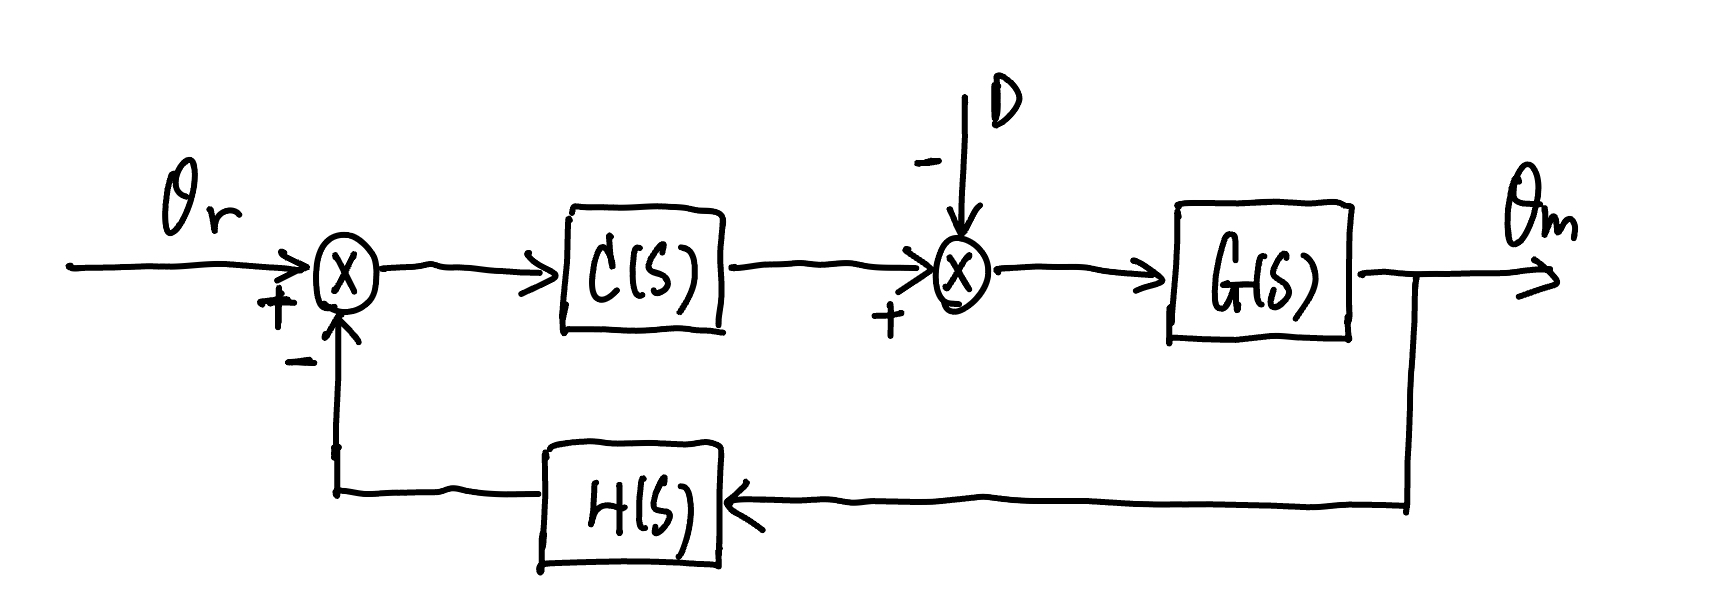
\includegraphics[max width=0.6\textwidth]{control/fd_control2.jpeg}
    \caption{A typical control system diagram}
    \label{fig:1}
\end{figure}


For the above control system, the forward path transfer function is $$
P(s)=C(s)G(s)
$$
The backward path transfer function is 
$$
H(s)
$$
The open loop transfer function is
$$
C(s)G(s)H(s)
$$
The input-to-output transfer function is 
$$
\frac{\Theta_m(s)}{\Theta_r(s)}=\frac{C(s)G(s)}{1+C(s)G(s)H(s)}
$$
The disturbance-to-output transfer function is 
$$
\frac{\Theta_m(s)}{D(s)}=\frac{G(s)}{1+C(s)G(s)H(s)}
$$

The input ($\theta_r$) to output ($\theta_m$) response of the closed-loop system will be determined by the roots of the characteristics equation
$$
1+C(s)G(s)H(s)=0
$$












\textbf{Background of final value theorem}

If a continuous signal $f(t)$ has its Laplace transformation $F(s)$, then the final value theorem states 

$$
\lim_{t\rightarrow\infty}f(t)=\lim_{s\rightarrow 0}sF(s)
$$






\section{Single Joint Position feedback}
The single joint motor system in Fig \ref{fig:motor_model2} is the plant we want to control. The plant transfer function $G(s)$ is (\ref{equ.motortf}), rewritten below
$$
G(s)=\frac{k_m}{s(1+T_ms)}
$$




We want to design a  proportional-integral controller 
$$
\begin{gathered}
C_{P}(s)=K_{P} \frac{1+s T_{P}}{s} 
\end{gathered}
$$
with $K_P$ and $T_P$ are design variable.

The control  diagram thus is shown below (note that the backward pass constant $k_{TP}$ is fixed).
\begin{figure}[H]
    \centering
    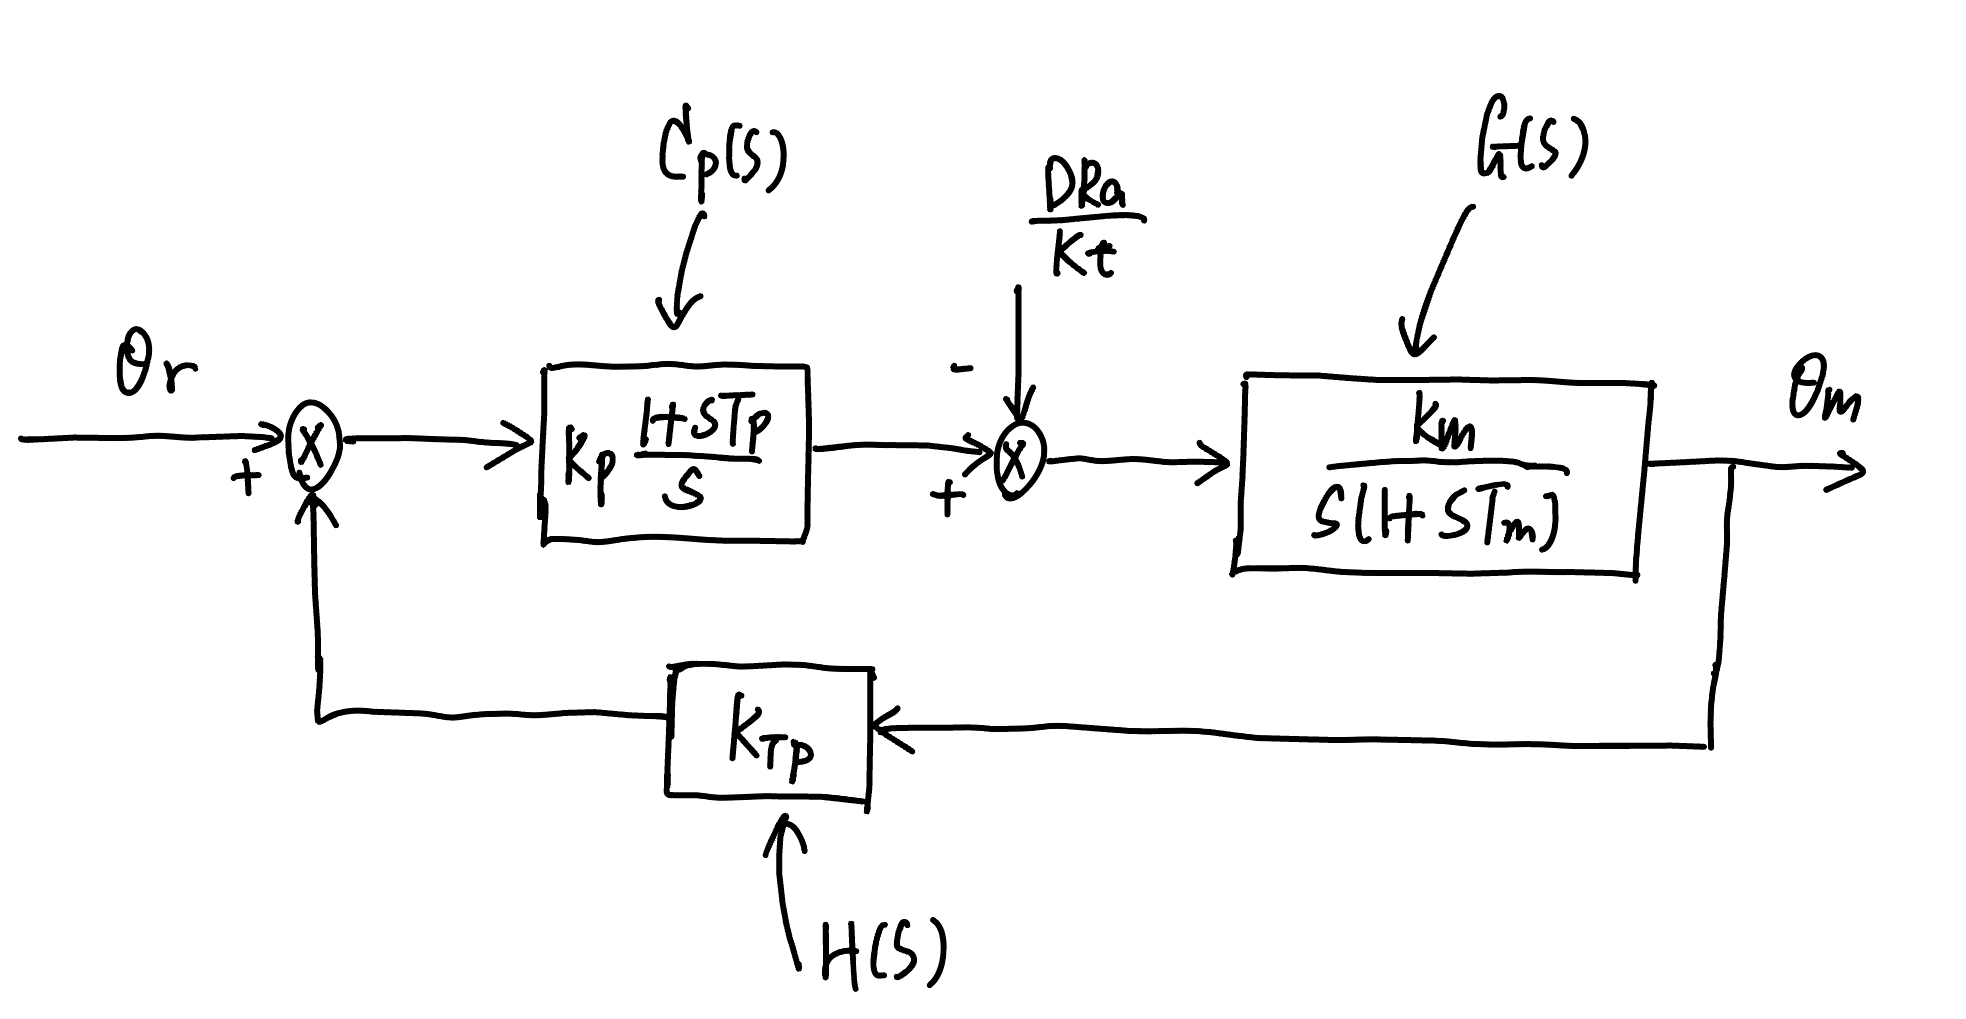
\includegraphics[max width=0.65\textwidth]{control/p_control2.jpg}
    \caption{Control diagram of position decentralized joint space control}
    \label{fig.p_control}
\end{figure}


The transfer function of the forward path is

$$
P(s)=G(s)C_P(s)=\frac{k_{m} K_{P}\left(1+s T_{P}\right)}{s^{2}\left(1+s T_{m}\right)}
$$

The transfer function of the backward pass is

$$
H(s)=k_{T P}
$$

The root locus  can be plotted as a function of the gain of the position loop $k_{m} K_{P} k_{T P} T_{P} / T_{m}$. Here, we derive into two cases to plot the root locus.

\begin{itemize}
    \item If $T_{P}<T_{m}$, the root locus is shown as below.  Thus, the system is inherently unstable.

    \begin{figure}[H]
    \centering
    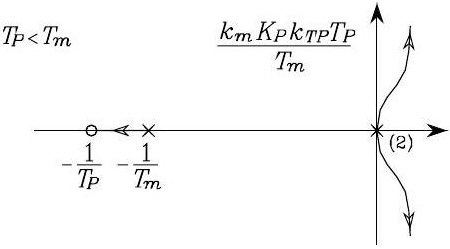
\includegraphics[max width=0.37\textwidth]{control/p_control_rl_1.jpg}
    \caption{Root locus when $T_{P}<T_{m}$}
    \label{fig.p_control_rl_1}
\end{figure}


 

    \item If $T_{P}>T_{m}$, the root locus is shown as below.  As $T_{P}$ increases, the absolute value of the real part of the two roots of the locus tending towards the asymptotes increases too, and the system has faster time response. 

        \begin{figure}[H]
    \centering
    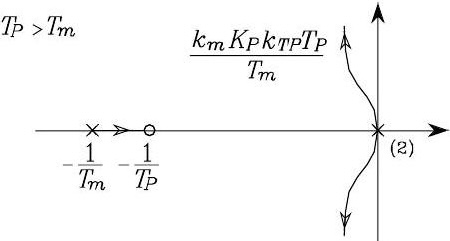
\includegraphics[max width=0.37\textwidth]{control/p_control_rl_2.jpg}
    \caption{Root locus when $T_{P}>T_{m}$}
    \label{fig.p_control_rl_2}
\end{figure}

\end{itemize}







The closed-loop input/output transfer function is

$$
\frac{\Theta_{m}(s)}{\Theta_{r}(s)}=\frac{P(s)}{1+P(s)H(s)}=\frac{{k_{m}K_P(1+T_Ps)}}{k_{TP}k_{m}K_P(1+T_Ps)+s^2(1+sT_m)},
$$

and the characteristic equation can be factorized into the following form


$$
{k_{TP}k_{m}K_P(1+T_Ps)+s^2(1+sT_m)}
=
{\left({\omega_{n}^{2}}+{2 \zeta }{\omega_{n}}s+{s^{2}}\right)(1+s \tau)}
$$


where $\omega_{n}$ and $\zeta$ are the natural frequency and damping ratio of the complex poles: $\left(-\zeta \omega_{n}, \pm j \sqrt{1-\zeta^{2}} \omega_{n}\right)$, and $-1 / \tau$ is the real pole. 
These poles correspond to the ones in the root locus in the above figures.




 The closed-loop disturbance/output transfer function is

$$
\frac{\Theta_{m}(s)}{D(s)}=-\frac{\frac{R_a}{K_t}G(s)}{1+P(s)H(s)}=-\frac{\frac{R_a}{K_t}k_ms}{k_{TP}k_{m}K_P(1+T_Ps)+s^2(1+sT_m)}
$$


If $\Theta_r(t)=0$, based on the final value theory, we have
\begin{equation}
    \lim_{t\rightarrow \infty} {\theta_{m}(t)}= \lim_{s\rightarrow 0} s{\Theta_{m}(s)}=\lim_{s\rightarrow 0} s\frac{\Theta_{m}(s)}{D(s)}{D(s)}
\end{equation}
thus,

\begin{equation}
    \lim_{t\rightarrow \infty} {\theta_{m}(t)}= 
    \begin{cases}
        0\qquad &\text{if}\quad D(t)\,\,\text{is constant signal}\\
        \frac{R_a}{K_t}\frac{1}{K_{P} k_{T P}} \qquad &\text{if}\quad D(t)\,\,\text{is ramp signal, such as $D(t)=vt$ }\\
    \end{cases}
\end{equation}

Hence, the controller can cancel the effect of constant disturbance, and the quantity

$$
K_{P} k_{T P}
$$

can be interpreted as the disturbance rejection factor for velocity (or higher-order) disturbance. Increasing  $K_{P}$ can help with reducing the effect of $D$, but too high $K_P$ can lead to unacceptable oscillations of the output, as implied from the root locus.

\section{Single-Joint Position and Velocity Feedback}
To control the motor system in Fig. \ref{fig:motor_model2},  we  use both  position and velocity controller
$$
\begin{gathered}
C_{P}(s)=K_{P} \quad \text{and} \quad C_{V}(s)=K_{V} \frac{1+s T_{V}}{s} 
\end{gathered}
$$
where $K_p$, $K_v$, and $T_v$ are the design variables.


The control diagram is shown below (Note that $k_{TV}$ and $k_{TP}$ in the backward pass are fixed).

\begin{figure}[H]
    \centering
    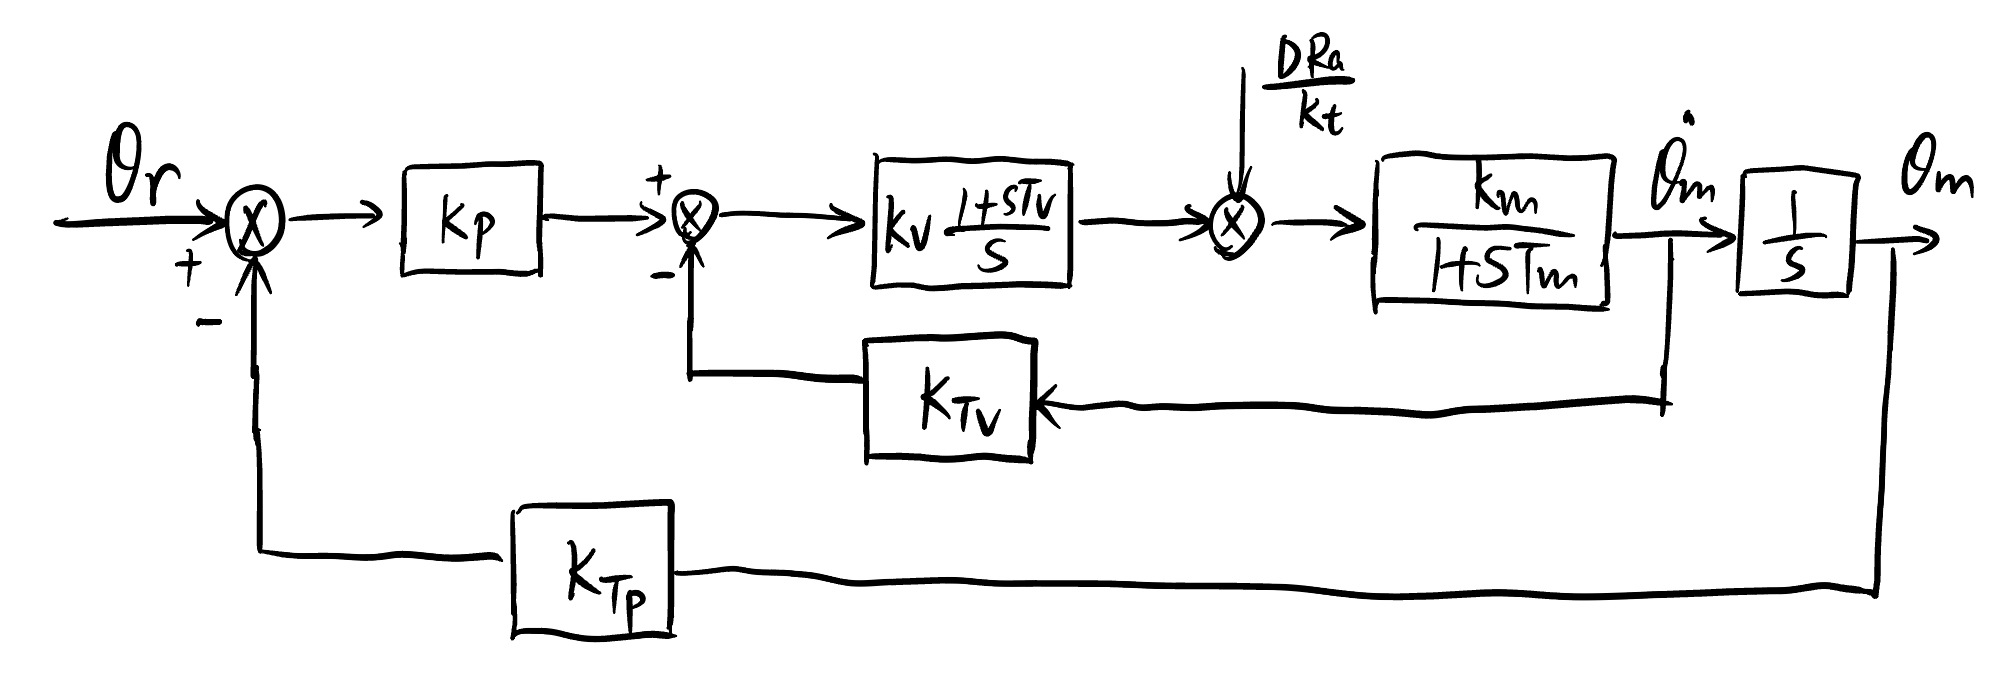
\includegraphics[max width=0.7\textwidth]{control/pv_control.jpeg}
    \caption{Control diagram of position and velocity control}
    \label{fig.pv_control}
\end{figure}

which can be further reduced into the following diagram:
\begin{figure}[H]
    \centering
    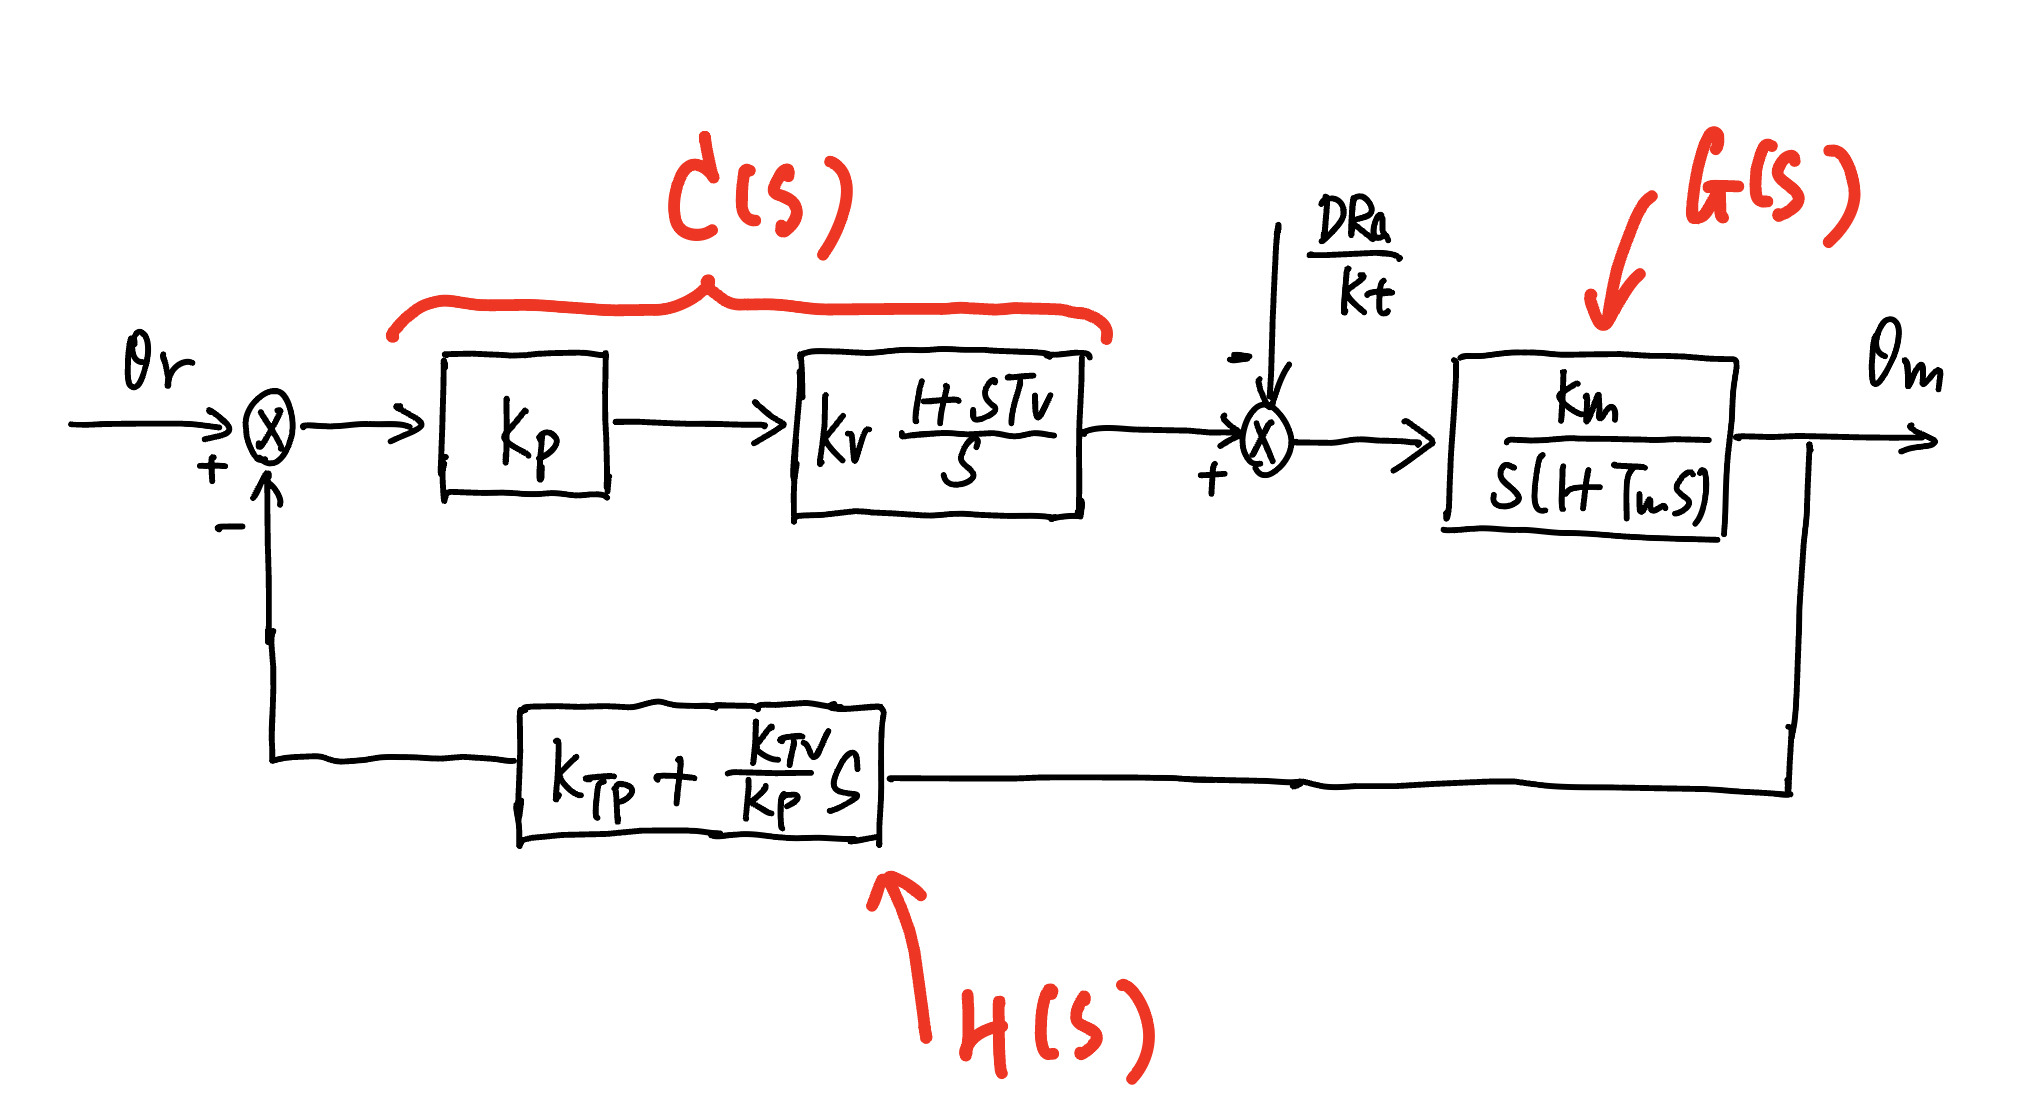
\includegraphics[max width=0.7\textwidth]{control/pv_control2.jpeg}
    \caption{Corresponding to Fig. \ref{fig.pv_control}, the equivalent control diagram}
    \label{fig.pv_control2}
\end{figure}


The transfer function of the forward path is

$$
P(s)=C(s)G(s)=\frac{k_{m} K_{P} K_{V}\left(1+s T_{V}\right)}{s^{2}\left(1+s T_{m}\right)}
$$






The transfer function of the backward path is

$$
H(s)=k_{T P}\left(1+s \frac{k_{T V}}{K_{P} k_{T P}}\right) .
$$


For simplicity, one can design $$
T_m=T_v,
$$ then that the poles of the closed-loop system move on the root locus as a function of the loop gain $k_{m} K_{V} k_{T V}$ is shown in the following figure:


        \begin{figure}[H]
    \centering
    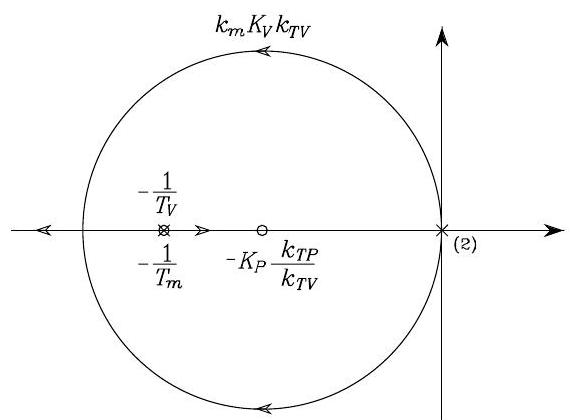
\includegraphics[max width=0.37\textwidth]{control/pv_control_rl_1.jpg}
    \caption{Root locus}
    \label{fig.pv_control_rl_1}
\end{figure}




By increasing the position  gain $K_{P}$, it is possible to confine the closed-loop poles into a region of the complex plane with large absolute values of the real part. 

The closed-loop input/output transfer function is

$$
\frac{\Theta_{m}(s)}{\Theta_{r}(s)}=\frac{C(s)G(s)}{1+C(s)G(s)H(s)}=\frac{\frac{1}{k_{T P}}}{1+\frac{s k_{T V}}{K_{P} k_{T P}}+\frac{s^{2}}{k_{m} K_{P} k_{T P} K_{V}}}=\frac{\frac{1}{k_{T P}}}{1+\frac{2 \zeta s}{\omega_{n}}+\frac{s^{2}}{\omega_{n}^{2}}}
$$



It can be recognized that, with a suitable choice of the gains, it is possible to obtain any value of natural frequency $\omega_{n}$ and damping ratio $\zeta$. Hence, if $\omega_{n}$ and $\zeta$ are given as design requirements, the following relations is

$$
K_{V} k_{T V}=\frac{2 \zeta \omega_{n}}{k_{m}}
$$




$$
K_{P} k_{T P} K_{V}=\frac{\omega_{n}^{2}}{k_{m}}
$$

For given transducer constants $k_{T P}$ and $k_{T V}$,  $K_{V}$ and $K_{P}$ can be chosen.
The closed-loop disturbance/output transfer function is

$$
\frac{\Theta_{m}(s)}{D(s)}=-\frac{\frac{R_a}{k_t}G(s)}{1+P(s)H(s)}=-\frac{\frac{R_a}{k_t}k_ms}{(1+sT_m)(s^2+k_mK_Vk_{TV}s+k_mK_PK_Vk_{TP})}
$$

which shows that the disturbance rejection factor is


If $\Theta_r(t)=0$, based on the final value theory, we have
\begin{equation}
    \lim_{t\rightarrow \infty} {\theta_{m}(t)}= \lim_{s\rightarrow 0} s{\Theta_{m}(s)}=\lim_{s\rightarrow 0} s\frac{\Theta_{m}(s)}{D(s)}{D(s)}
\end{equation}
thus,

\begin{equation}
    \lim_{t\rightarrow \infty} {\theta_{m}(t)}= 
    \begin{cases}
        0\qquad &\text{if}\quad D(t)\,\,\text{is constant signal}\\
        \frac{R_a}{k_t}\frac{1}{K_{P} k_{T P} K_{V}} \qquad &\text{if}\quad D(t)\,\,\text{is ramp signal, such as $D(t)=vt$ }\\
    \end{cases}
\end{equation}

Hence, the controller can cancel the effect of constant disturbance, and the quantity

$$
K_{P} k_{T P} K_{V}
$$

can be interpreted as the disturbance rejection factor for velocity (or higher-order) disturbance. Increasing  $K_{P}$ and $K_V$ can help with reducing the effect of $D$.




 
% \section{Position, velocity and acceleration feedback (optional)}
% In this case, the control action is characterized by

% $$
% C_{P}(s)=K_{P} \quad C_{V}(s)=K_{V} \quad C_{A}(s)=K_{A} \frac{1+s T_{A}}{s}
% $$

% Define

% $$
% G^{\prime}(s)=\frac{k_{m}}{\left(1+k_{m} K_{A} k_{T A}\right)\left(1+\frac{s T_{m}\left(1+k_{m} K_{A} k_{T A} \frac{T_{A}}{T_{m}}\right)}{\left(1+k_{m} K_{A} k_{T A}\right)}\right)}
% $$

% The transfer function of the forward path is

% $$
% P(s)=\frac{K_{P} K_{V} K_{A}\left(1+s T_{A}\right)}{s^{2}} G^{\prime}(s)
% $$

% while that of the return path is

% $$
% H(s)=k_{T P}\left(1+\frac{s k_{T V}}{K_{P} k_{T P}}\right) .
% $$

% In this case, a suitable pole cancellation is worthy which can be achieved either by setting

% $$
% T_{A}=T_{m}
% $$

% or by making

% $$
% k_{m} K_{A} k_{T A} T_{A} \gg T_{m} \quad k_{m} K_{A} k_{T A} \gg 1
% $$



% The two solutions are equivalent as regards dynamic performance of the control system. In both cases, the poles of the closed-loop system are constrained to move on the root locus as a function of the loop gain $k_{m} K_{P} K_{V} K_{A} /(1+$ $k_{m} K_{A} k_{T A}$ ). A close analogy with the previous scheme can be recognized, in that the resulting closed-loop system is again of second-order type.

% The closed-loop input/output transfer function is

% $$
% \frac{\Theta_{m}(s)}{\Theta_{r}(s)}=\frac{\frac{1}{k_{T P}}}{1+\frac{s k_{T V}}{K_{P} k_{T P}}+\frac{s^{2}\left(1+k_{m} K_{A} k_{T A}\right)}{k_{m} K_{P} k_{T P} K_{V} K_{A}}},
% $$

% while the closed-loop disturbance/output transfer function is

% $$
% \frac{\Theta_{m}(s)}{D(s)}=-\frac{\frac{s R_{a}}{k_{t} K_{P} k_{T P} K_{V} K_{A}\left(1+s T_{A}\right)}}{1+\frac{s k_{T V}}{K_{P} k_{T P}}+\frac{s^{2}\left(1+k_{m} K_{A} k_{T A}\right)}{k_{m} K_{P} k_{T P} K_{V} K_{A}}} .
% $$

% The resulting disturbance rejection factor is given by

% $$
% X_{R}=K_{P} k_{T P} K_{V} K_{A}
% $$






\end{document}